\documentclass[12pt,letterpaper]{article}

% just for the example
\usepackage{lipsum}
% Set margins to 1.5in
\usepackage[margin=1.5in]{geometry}

% for graphics
\usepackage{graphicx}
\graphicspath{{./figures/}}

% for crimson text
\usepackage{crimson}
\usepackage[T1]{fontenc}

% setup parameter indentation
\setlength{\parindent}{0pt}
\setlength{\parskip}{6pt}

% for 1.15 spacing between text
\renewcommand{\baselinestretch}{1.15}

% For defining spacing between headers
\usepackage{titlesec}
% Level 1
\titleformat{\section}
  {\normalfont\fontsize{18}{0}\bfseries}{\thesection}{1em}{}
% Level 2
\titleformat{\subsection}
  {\normalfont\fontsize{14}{0}\bfseries}{\thesection}{1em}{}
% Level 3
\titleformat{\subsubsection}
  {\normalfont\fontsize{12}{0}\bfseries}{\thesection}{1em}{}
% Level 4
\titleformat{\paragraph}
  {\normalfont\fontsize{12}{0}\bfseries\itshape}{\theparagraph}{1em}{}
% Level 5
\titleformat{\subparagraph}
  {\normalfont\fontsize{12}{0}\itshape}{\theparagraph}{1em}{}
% Level 6
\makeatletter
\newcounter{subsubparagraph}[subparagraph]
\renewcommand\thesubsubparagraph{%
  \thesubparagraph.\@arabic\c@subsubparagraph}
\newcommand\subsubparagraph{%
  \@startsection{subsubparagraph}    % counter
    {6}                              % level
    {\parindent}                     % indent
    {12pt} % beforeskip
    {6pt}                           % afterskip
    {\normalfont\fontsize{12}{0}}}
\newcommand\l@subsubparagraph{\@dottedtocline{6}{10em}{5em}}
\newcommand{\subsubparagraphmark}[1]{}
\makeatother
\titlespacing*{\section}{0pt}{12pt}{6pt}
\titlespacing*{\subsection}{0pt}{12pt}{6pt}
\titlespacing*{\subsubsection}{0pt}{12pt}{6pt}
\titlespacing*{\paragraph}{0pt}{12pt}{6pt}
\titlespacing*{\subparagraph}{0pt}{12pt}{6pt}
\titlespacing*{\subsubparagraph}{0pt}{12pt}{6pt}

% Set caption to correct size and location
\usepackage[tableposition=top, figureposition=bottom, font=footnotesize, labelfont=bf]{caption}

% set page number location
\usepackage{fancyhdr}
\fancyhf{} % clear all header and footers
\renewcommand{\headrulewidth}{0pt} % remove the header rule
\rhead{\thepage}
\pagestyle{fancy}

% Overwrite Title
\makeatletter
\renewcommand{\maketitle}{\bgroup
   \begin{center}
   \textbf{{\fontsize{18pt}{20}\selectfont \@title}}\\
   \vspace{10pt}
   {\fontsize{12pt}{0}\selectfont \@author} 
   \end{center}
}
\makeatother

% Used for Tables and Figures
\usepackage{float}

% For using lists
\usepackage{enumitem}

% For using APA Citation format
\usepackage{apacite}

% Custom Quote
\newenvironment{myquote}[1]%
  {\list{}{\leftmargin=#1\rightmargin=#1}\item[]}%
  {\endlist}
  
% Create Abstract 
\renewenvironment{abstract}
{\vspace*{-.5in}\fontsize{12pt}{12}\begin{myquote}{.5in}
\noindent \par{\bfseries \abstractname.}}
{\medskip\noindent
\end{myquote}
}

\begin{document}

% Set Title, Author, and email
\title{Assignment M1}
\author{Snejana Shegheva \\ sshegheva3@gatech.edu}

\maketitle
\thispagestyle{fancy}

\begin{abstract}
Mapping data from one form to another for its ease-of-use is at the core of the \textit{Extract, Transform and Load} process. There exist many tools that can accomplish the task of creating and maintaining a data warehouse. However, sometimes it is advantageous to have a custom solution that allows user to interact with the data directly during some or all of the ETL phases. In this project, we analyze an internal interface of a \textit{transform} task that prepares the data for use in a personalized recommendation system powered by Artificial Intelligence engines. 
\end{abstract}

\section*{Problem Space}
The data ingestion is described by the \textit{Extract, Transform and Load} (ETL) process - a cycle that converts a raw data into structured records more convenient for further Data Analysis and/or use for Machine Learning algorithms \cite{wiki:xxx}. Figure~\ref{fig::1} shows the ETL process from the Source to the Destination. The entire cycle may be completely hidden from the user (full automation of data ingestion), or a human is required to guide the components of the process to reach their desired goal. In this project we focus on the \textit{transform} task that is centered around interactions with the user to alter the original data to meet their needs. For example, a user who looks at the weather feed in Fahrenheit may choose to convert it to Celsius. 

\begin{figure}[H]
\centering
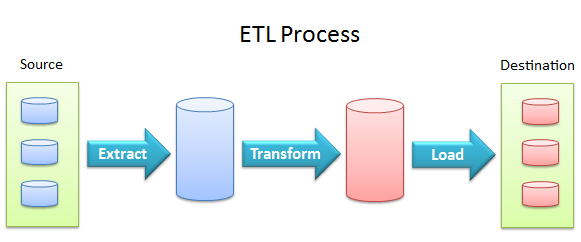
\includegraphics[width=3in, scale=.3]{ETLProcess.png}
\caption{Extract-Transform-Load Process from Data Science Central blogpost on Open Source ETL tools (https://www.datasciencecentral.com/profiles/blogs/10-open-source-etl-tools)}
\label{fig::1}
\end{figure}

To accomplish the data transformation task, a user needs an access to the original data, as well as an arsenal of mapping tools suitable to the domain. 

\section*{User Types}
\lipsum[1]

\section*{Needfinding Plan 1}
\lipsum[1]

\section*{Needfinding Plan 2}

\lipsum[1]
\section*{Needfinding Plan 3}
\lipsum[1]


\bibliographystyle{apacite} 
\bibliography{bibtemp}

\end{document}
